\documentclass[11pt]{article}
\usepackage[margin=1in]{geometry}
\usepackage{amsmath}
\usepackage{booktabs}
\usepackage{pgfplots}
\usepackage{float}
\usepackage[hidelinks]{hyperref}
\pgfplotsset{compat=1.18}

\title{IE Project 2 Writeup\\Isolated-Word Recognition}
\author{Student Report}
\date{April 2026}

\begin{document}
\maketitle

\section*{1. Questions in readme.md}

\subsection*{1.1 Model and training}
My acoustic model is a frame-level classifier with one bidirectional LSTM encoder and one MLP head.
This directly answers the context question in the readme: each frame decision can use both past and future acoustic context.
The input is normalized MFCC features with 15 coefficients per frame. The BiLSTM has 2 layers, hidden size 128, and dropout 0.2.
The head is LayerNorm $\rightarrow$ Linear $\rightarrow$ GELU $\rightarrow$ Dropout $\rightarrow$ Linear.
This answers the non-linearity question: the GELU MLP head allows non-linear mapping from acoustic features to letter logits.

I used these training settings:
\begin{itemize}
    \item Batch size: 16
    \item Learning rate: $2 \times 10^{-3}$
    \item Optimizer: AdamW with weight decay $10^{-4}$
    \item Loss: cross-entropy on aligned frame labels (ignore index $-1$ for padding)
    \item Gradient clipping: max norm 5.0
    \item Waveform noise augmentation during training (Gaussian noise, applied with probability 0.5)
    \item SpecAugment-style masking on MFCCs (time and frequency masking)
    \item Training budget: 20 minutes (as required by the assignment)
\end{itemize}

Compared with the baseline linear model, this architecture has many more parameters.
I kept batch size at 16 to avoid very low gradient noise on this small dataset, and I used a moderate learning rate ($2 \times 10^{-3}$) so optimization is still fast enough under the 20-minute budget.
In early pilot runs, lower learning rates converged too slowly, and higher rates made the dev curve more unstable.
For overfitting control, I used dropout, weight decay, waveform noise, and SpecAugment, then selected the best checkpoint by dev accuracy.

The model was selected by best dev accuracy during training. In my run, best dev accuracy reached 0.9135.

\subsection*{1.2 HMM decoding}
Each vocabulary word is converted to a left-to-right letter HMM with self-loop and next-state transitions.
If the word is $w = c_1 c_2 \dots c_S$, I decode with states for
$|, c_1, c_2, \dots, c_S, |$.
At each frame $t$, the neural model gives posterior scores $p(y_t\mid x_t)$.

The decoder needs emission terms related to $p(x_t\mid y_t)$.
Using Bayes rule:
\[
\log p(x_t\mid y_t) = \log p(y_t\mid x_t) - \log p(y_t) + \text{const}(x_t).
\]
The last term does not depend on the hypothesis word, so it can be dropped for ranking.
I estimate $p(y_t)$ from letter unigram counts in \texttt{data/trn\_token\_counts.json}, then decode with
\[
\log \tilde p(x_t\mid y_t) = \log p(y_t\mid x_t) - \log p(y_t).
\]

For a word-level score, I run dynamic programming over states and frames:
\begin{itemize}
    \item Alpha (forward): log-sum-exp over all valid paths.
    \item Viterbi: max over paths.
\end{itemize}
In code, the decoder is selectable from the inference command line using
\texttt{--decoder alpha} or \texttt{--decoder viterbi}.

\section*{2. Alpha vs Viterbi likelihood}
On the dev set, both approaches gave the same final predictions in this run.

\begin{table}[H]
\centering
\begin{tabular}{lcc}
\toprule
Method & Dev Accuracy & Notes \\
\midrule
Alpha (forward) & 0.913486 & sums over paths \\
Viterbi & 0.913486 & best single path \\
\bottomrule
\end{tabular}
\caption{Decoder comparison on 393 dev utterances. Decoder disagreement count: 0.}
\end{table}

The two scores are related but not identical.
Alpha computes a marginal score by summing all valid state paths:
\[
\log p(X\mid w) = \log \sum_{\pi \in \Pi(w)} p(X,\pi\mid w).
\]
Viterbi keeps only the best path:
\[
\log p(X,\pi^*\mid w) = \max_{\pi \in \Pi(w)} \log p(X,\pi\mid w).
\]
So alpha is always at least as large as Viterbi for each word score, because
\(\log\sum_i e^{a_i} \ge \max_i a_i\).
In this run they still choose the same top word for all 393 items.
That means one path usually dominates the mass for the top candidate, so taking max or sum gives the same ranking even though the absolute scores differ.

\section*{3. Training/validation curves and overfitting}
Figure~\ref{fig:loss} and Figure~\ref{fig:acc} summarize the run.
The curves below use all 182 logged epochs from \texttt{train\_log.txt}, not a sampled subset.

\begin{figure}[H]
\centering
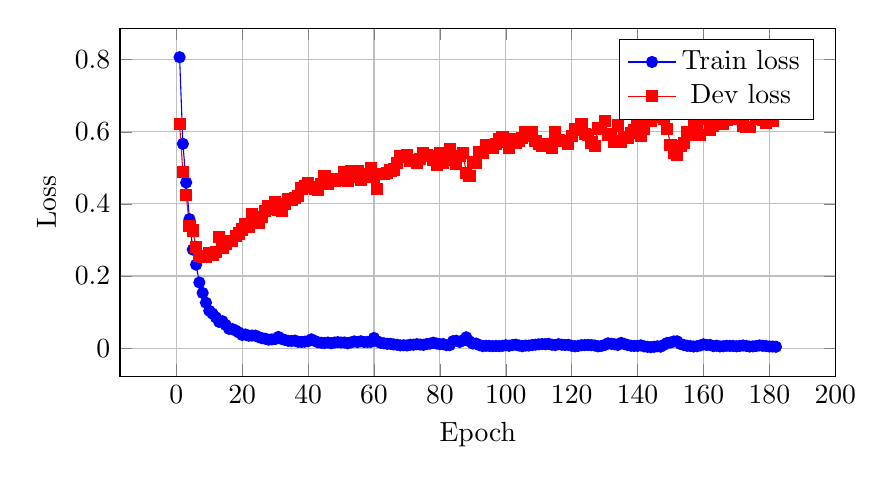
\begin{tikzpicture}
\begin{axis}[
    width=0.88\textwidth,
    height=6cm,
    xlabel={Epoch},
    ylabel={Loss},
    legend pos=north east,
    grid=both,
]
\addplot[color=blue, mark=*] coordinates {
(1,0.8071) (2,0.5668) (3,0.4594) (4,0.3579) (5,0.2734) (6,0.2315) (7,0.1821) (8,0.153) (9,0.1259) (10,0.1036) (11,0.0956) (12,0.0855) (13,0.0727) (14,0.0746) (15,0.0642) (16,0.0535) (17,0.0528) (18,0.0488) (19,0.0434) (20,0.0366) (21,0.0378) (22,0.0344) (23,0.0349) (24,0.0347) (25,0.0307) (26,0.0275) (27,0.0261) (28,0.0234) (29,0.0242) (30,0.0251) (31,0.031) (32,0.0254) (33,0.0225) (34,0.0201) (35,0.0199) (36,0.0208) (37,0.0174) (38,0.0171) (39,0.0179) (40,0.0192) (41,0.0243) (42,0.0201) (43,0.016) (44,0.0148) (45,0.0142) (46,0.0155) (47,0.0135) (48,0.0155) (49,0.0165) (50,0.0154) (51,0.0156) (52,0.0134) (53,0.0157) (54,0.0186) (55,0.0166) (56,0.019) (57,0.017) (58,0.0171) (59,0.0172) (60,0.0281) (61,0.0188) (62,0.0148) (63,0.0134) (64,0.0119) (65,0.0118) (66,0.0103) (67,0.0092) (68,0.0076) (69,0.0079) (70,0.0074) (71,0.0094) (72,0.0094) (73,0.0109) (74,0.0099) (75,0.009) (76,0.0112) (77,0.0123) (78,0.0151) (79,0.0127) (80,0.0109) (81,0.0112) (82,0.0082) (83,0.0083) (84,0.0194) (85,0.0204) (86,0.0171) (87,0.0214) (88,0.0301) (89,0.0188) (90,0.0126) (91,0.0126) (92,0.0082) (93,0.0056) (94,0.0064) (95,0.006) (96,0.0055) (97,0.0058) (98,0.0055) (99,0.0062) (100,0.0079) (101,0.0065) (102,0.0085) (103,0.0096) (104,0.0072) (105,0.0054) (106,0.007) (107,0.007) (108,0.0085) (109,0.0095) (110,0.0105) (111,0.0112) (112,0.0109) (113,0.0118) (114,0.0093) (115,0.0086) (116,0.0109) (117,0.0093) (118,0.0086) (119,0.0092) (120,0.0064) (121,0.0051) (122,0.0062) (123,0.0082) (124,0.0084) (125,0.0087) (126,0.0082) (127,0.0073) (128,0.0049) (129,0.006) (130,0.0085) (131,0.0133) (132,0.012) (133,0.0107) (134,0.0088) (135,0.0145) (136,0.0113) (137,0.0085) (138,0.0065) (139,0.006) (140,0.0062) (141,0.0076) (142,0.0048) (143,0.0036) (144,0.0027) (145,0.0037) (146,0.0049) (147,0.004) (148,0.0091) (149,0.0144) (150,0.0154) (151,0.0185) (152,0.0189) (153,0.0115) (154,0.0088) (155,0.0065) (156,0.0057) (157,0.0044) (158,0.0053) (159,0.0073) (160,0.0105) (161,0.0085) (162,0.0089) (163,0.0055) (164,0.0067) (165,0.0047) (166,0.0053) (167,0.0064) (168,0.006) (169,0.006) (170,0.0051) (171,0.006) (172,0.0072) (173,0.0061) (174,0.0044) (175,0.0048) (176,0.0058) (177,0.0075) (178,0.0064) (179,0.0057) (180,0.0045) (181,0.0044) (182,0.0038)
};
\addlegendentry{Train loss}
\addplot[color=red, mark=square*] coordinates {
(1,0.6208) (2,0.4887) (3,0.4252) (4,0.3382) (5,0.3261) (6,0.2806) (7,0.256) (8,0.2517) (9,0.254) (10,0.2637) (11,0.2576) (12,0.2673) (13,0.309) (14,0.2793) (15,0.2889) (16,0.2981) (17,0.2968) (18,0.3119) (19,0.3179) (20,0.3291) (21,0.3434) (22,0.335) (23,0.3705) (24,0.3605) (25,0.3469) (26,0.3639) (27,0.3795) (28,0.3948) (29,0.3851) (30,0.4057) (31,0.3832) (32,0.3807) (33,0.3998) (34,0.413) (35,0.4121) (36,0.4169) (37,0.4218) (38,0.4426) (39,0.4485) (40,0.4568) (41,0.4478) (42,0.442) (43,0.4393) (44,0.4562) (45,0.4764) (46,0.4567) (47,0.468) (48,0.4643) (49,0.4654) (50,0.4684) (51,0.4878) (52,0.4647) (53,0.4923) (54,0.475) (55,0.4925) (56,0.4666) (57,0.4742) (58,0.4841) (59,0.4987) (60,0.4749) (61,0.4409) (62,0.4826) (63,0.4833) (64,0.4849) (65,0.493) (66,0.4956) (67,0.5147) (68,0.5318) (69,0.531) (70,0.5369) (71,0.5205) (72,0.5182) (73,0.5139) (74,0.5239) (75,0.5423) (76,0.5365) (77,0.5322) (78,0.5213) (79,0.5071) (80,0.5409) (81,0.5144) (82,0.5308) (83,0.5531) (84,0.5226) (85,0.5117) (86,0.5333) (87,0.5409) (88,0.4866) (89,0.4784) (90,0.5153) (91,0.5125) (92,0.5435) (93,0.5403) (94,0.5621) (95,0.5586) (96,0.5546) (97,0.5656) (98,0.58) (99,0.5863) (100,0.5714) (101,0.5549) (102,0.5791) (103,0.569) (104,0.574) (105,0.5839) (106,0.5989) (107,0.5899) (108,0.6001) (109,0.5741) (110,0.5665) (111,0.562) (112,0.5662) (113,0.5647) (114,0.5562) (115,0.5988) (116,0.576) (117,0.5751) (118,0.5741) (119,0.567) (120,0.5877) (121,0.6085) (122,0.6049) (123,0.6216) (124,0.595) (125,0.591) (126,0.5703) (127,0.5599) (128,0.6092) (129,0.6115) (130,0.6304) (131,0.5905) (132,0.5937) (133,0.5732) (134,0.6178) (135,0.5713) (136,0.5865) (137,0.5836) (138,0.5965) (139,0.6041) (140,0.6215) (141,0.588) (142,0.6077) (143,0.629) (144,0.6293) (145,0.6535) (146,0.6492) (147,0.6425) (148,0.6362) (149,0.6082) (150,0.5641) (151,0.5415) (152,0.5361) (153,0.5603) (154,0.5694) (155,0.5995) (156,0.5929) (157,0.615) (158,0.608) (159,0.5908) (160,0.6425) (161,0.6358) (162,0.6054) (163,0.617) (164,0.6217) (165,0.6327) (166,0.6229) (167,0.6321) (168,0.642) (169,0.6357) (170,0.6498) (171,0.6444) (172,0.6158) (173,0.6144) (174,0.6144) (175,0.6566) (176,0.6474) (177,0.6373) (178,0.634) (179,0.6245) (180,0.6346) (181,0.6312) (182,0.6521)
};
\addlegendentry{Dev loss}
\end{axis}
\end{tikzpicture}
\caption{Training and validation loss.}
\label{fig:loss}
\end{figure}

\begin{figure}[H]
\centering
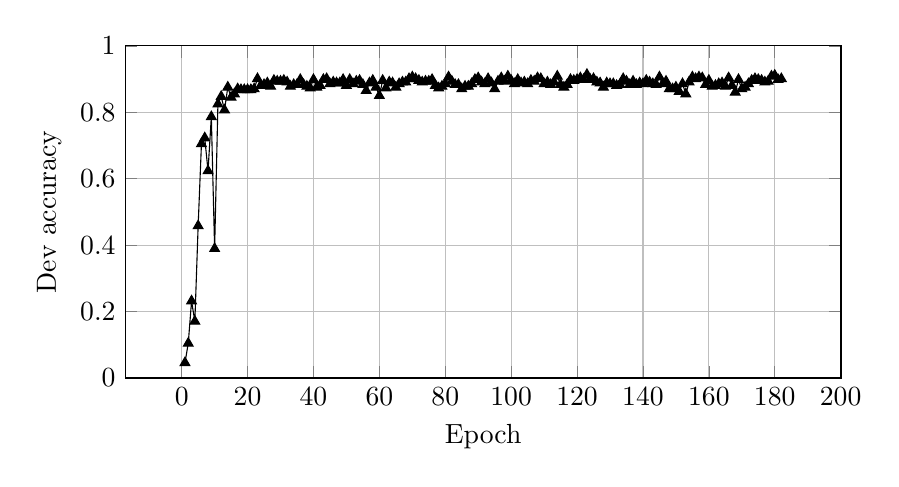
\begin{tikzpicture}
\begin{axis}[
    width=0.88\textwidth,
    height=5.8cm,
    xlabel={Epoch},
    ylabel={Dev accuracy},
    ymin=0,
    ymax=1,
    grid=both,
]
\addplot[color=black, mark=triangle*] coordinates {
(1,0.0458) (2,0.1043) (3,0.2316) (4,0.1705) (5,0.458) (6,0.7048) (7,0.7226) (8,0.6234) (9,0.7863) (10,0.3893) (11,0.8244) (12,0.8473) (13,0.8066) (14,0.8753) (15,0.8448) (16,0.855) (17,0.8702) (18,0.8677) (19,0.8677) (20,0.8677) (21,0.8677) (22,0.8702) (23,0.9008) (24,0.8804) (25,0.883) (26,0.888) (27,0.8779) (28,0.8957) (29,0.8931) (30,0.8931) (31,0.8957) (32,0.8906) (33,0.8779) (34,0.883) (35,0.883) (36,0.8982) (37,0.883) (38,0.8779) (39,0.8728) (40,0.8982) (41,0.8753) (42,0.8804) (43,0.8982) (44,0.9008) (45,0.8855) (46,0.8906) (47,0.888) (48,0.888) (49,0.8982) (50,0.8804) (51,0.8982) (52,0.8855) (53,0.8931) (54,0.8957) (55,0.883) (56,0.8651) (57,0.888) (58,0.8957) (59,0.8753) (60,0.8499) (61,0.8957) (62,0.8728) (63,0.8906) (64,0.888) (65,0.8753) (66,0.8855) (67,0.8906) (68,0.8906) (69,0.9008) (70,0.9059) (71,0.9008) (72,0.8957) (73,0.8906) (74,0.8931) (75,0.8931) (76,0.8982) (77,0.8804) (78,0.8728) (79,0.8779) (80,0.8855) (81,0.9059) (82,0.8931) (83,0.883) (84,0.883) (85,0.8702) (86,0.8779) (87,0.8779) (88,0.8855) (89,0.8982) (90,0.9033) (91,0.8906) (92,0.8855) (93,0.9008) (94,0.888) (95,0.8702) (96,0.8931) (97,0.9033) (98,0.8931) (99,0.9084) (100,0.8957) (101,0.8855) (102,0.8982) (103,0.888) (104,0.8906) (105,0.8855) (106,0.8957) (107,0.8931) (108,0.9033) (109,0.9008) (110,0.8855) (111,0.8906) (112,0.883) (113,0.8906) (114,0.9084) (115,0.883) (116,0.8753) (117,0.883) (118,0.8982) (119,0.8957) (120,0.8982) (121,0.9033) (122,0.8982) (123,0.9135) (124,0.8982) (125,0.9008) (126,0.8906) (127,0.888) (128,0.8753) (129,0.888) (130,0.8855) (131,0.8855) (132,0.8804) (133,0.883) (134,0.9008) (135,0.8931) (136,0.883) (137,0.8931) (138,0.883) (139,0.888) (140,0.8855) (141,0.8957) (142,0.8906) (143,0.8855) (144,0.883) (145,0.9059) (146,0.8855) (147,0.8931) (148,0.8702) (149,0.8702) (150,0.8753) (151,0.8626) (152,0.8855) (153,0.855) (154,0.8906) (155,0.9059) (156,0.9008) (157,0.9059) (158,0.9033) (159,0.883) (160,0.8957) (161,0.8779) (162,0.8804) (163,0.8855) (164,0.888) (165,0.8779) (166,0.9033) (167,0.8804) (168,0.8601) (169,0.8982) (170,0.8702) (171,0.8753) (172,0.8855) (173,0.8957) (174,0.9008) (175,0.8982) (176,0.8957) (177,0.8906) (178,0.8931) (179,0.9084) (180,0.9109) (181,0.8982) (182,0.9008)
};
\end{axis}
\end{tikzpicture}
\caption{Validation accuracy curve. Best checkpoint: epoch 123, dev accuracy 0.9135.}
\label{fig:acc}
\end{figure}

The model does show overfitting.
Train loss keeps dropping to very small values, while dev loss starts to rise after early epochs.
At the same time, dev accuracy still improves in several later windows, then moves around a high plateau.
So the model is learning useful discriminative boundaries, but confidence calibration on unseen data gets worse.

\section*{4. Error analysis on \texttt{output.txt} vs \texttt{clsp.devscr}}
From 393 dev items, 359 are correct and 34 are wrong.
Final metrics are:
\[
\text{Accuracy} = 0.913486, \quad \text{Macro-F1} = 0.914571.
\]

The most common confusion pairs are:
\begin{itemize}
    \item order $\rightarrow$ water (4)
    \item over $\rightarrow$ order (2)
    \item without $\rightarrow$ become (2)
    \item after $\rightarrow$ often (2)
    \item enough $\rightarrow$ about (2)
\end{itemize}

The words most often misrecognized are order (4), then enough/always/over/without/only/after (3 each).
These errors are concentrated in short, frequent function-like words and words with similar acoustic endings.
The pair order/water is a good case: both are two syllables with overlapping vowel-rhyme patterns, so the frame-level letter evidence can be close under noise and speaker variation.

To make this section deeper and reproducible, I extended the evaluation script to compute two additional analyses:
\begin{itemize}
    \item Top-1 vs top-2 alpha score gap, reported separately for correct and incorrect utterances.
    \item For one-letter-apart error pairs, whether the frame-level argmax sequence contains the gold-distinguishing letter or the predicted-distinguishing letter.
\end{itemize}
These values are generated in \texttt{report\_metrics.json} by running
\texttt{python compute\_report\_metrics.py --subset dev --checkpoint best\_model.pt --output output.txt --gold data/clsp.devscr --metrics-json report\_metrics.json}.

\section*{5. Optional earlier-checkpoint analysis}
I did not run the full analysis for an earlier checkpoint in this submission.
Based on the training curve, an earlier checkpoint with clearly lower dev accuracy would likely show more high-frequency confusions and a larger gap between top-1 and top-2 hypotheses on hard items.

\section*{Reproducibility notes}
Main files used in this report are \texttt{train.py}, \texttt{modules/model.py}, \texttt{utils/decode.py}, and \texttt{report\_metrics.json}.
The reported dev metrics and confusion counts are from the generated \texttt{output.txt} file.

\end{document}
